\documentclass{article}
\usepackage{tikz}
\usetikzlibrary{positioning,shapes}

\begin{document}

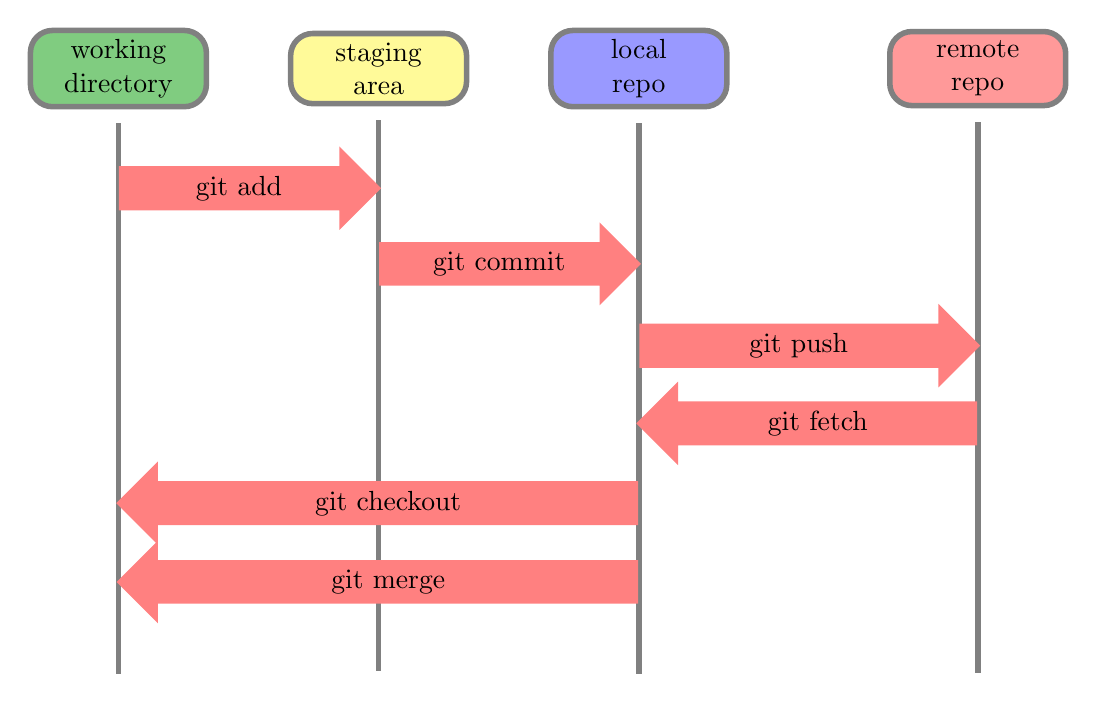
\begin{tikzpicture}[head/.style={line width=2pt,draw=gray,rounded corners=8pt,text width=2cm,align=center}]
\node[head,fill=green!60!black!50] (wd) {working directory};
\node[head,fill=yellow!40,right=of wd] (sa) {staging \\ area};
\node[head,fill=blue!40,right=of sa] (lr) {local \\ repo};
\node[head,fill=red!40,right=2cm of lr] (rr) {remote \\ repo};
\begin{scope}[line width=2pt,gray]
\foreach \x in {wd,sa,lr,rr}
  \draw ([yshift=-5pt]\x.south) -- +(0,-7cm);
\end{scope}
\begin{scope}[every node/.style={single arrow, draw=none,fill=red!50,anchor=west,align=center}]
\node [anchor=west,text width=2.8cm] at ([yshift=-1cm]wd.south) {git add};
\node [anchor=west,text width=2.8cm] at ([yshift=-2cm]sa.south) {git commit};
\node [anchor=west,text width=3.8cm] at ([yshift=-3cm]lr.south) {git push};
\node [anchor=east,text width=3.8cm,shape border rotate=180] at ([yshift=-4cm]rr.south) {git fetch};
\node [anchor=east,text width=6.1cm,shape border rotate=180] at ([yshift=-5cm]lr.south) {git checkout};
\node [anchor=east,text width=6.1cm,shape border rotate=180] at ([yshift=-6cm]lr.south) {git merge};
\end{scope}
\end{tikzpicture}
\end{document}
